\documentclass[aspectratio=169,12pt]{beamer}
%\documentclass{beamer}
\usepackage{graphicx,url,pbox,hyperref, verbatim, minted}
\usepackage{colortbl}
\usetheme{Copenhagen}
\usecolortheme{crane}
\setbeamerfont{frametitle}{size=\normalsize}
\setbeamertemplate{footline}[frame number]

\title{\normalsize Capstone ideas.}

\author{David Tersegno\\\scriptsize DSIR 222}

\setbeamercovered{transparent}
\beamertemplatenavigationsymbolsempty
%or 
%\setbeamertemplate{navigation symbols}{}
\date{April 18, 2022}


\begin{document}
	
	\begin{frame}
		\maketitle
	\end{frame}


	\begin{frame}
		\frametitle{Cardle}
		A Wordle meta-game\\
		\vfill\vfill\strut\\
		\begin{tabular}{ccp{120pt}}
			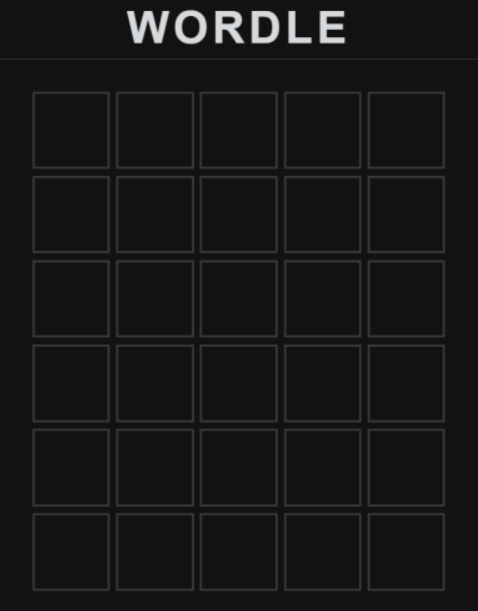
\includegraphics[width=0.3\linewidth, trim = 0 80pt 0 80pt]{pix/wordleSS}	&	
			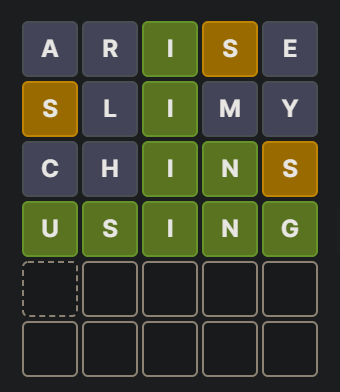
\includegraphics[width=0.3\linewidth, trim =0 60pt 0 60pt]{pix/wordplay}&
			Make a card game out of Wordle games shared on Twitter and Slack. Train models to make good decisions.
		\end{tabular}
	\end{frame}
	\begin{frame}
\frametitle{Cardle}
\hfill
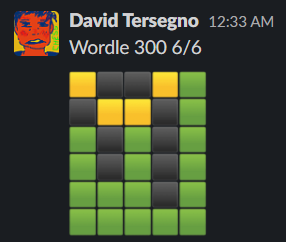
\includegraphics[width=0.2\linewidth]{pix/david}\hfill
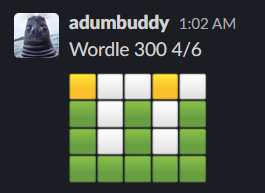
\includegraphics[width=0.2\linewidth]{pix/adam}\hfill
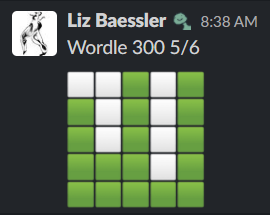
\includegraphics[width=0.2\linewidth]{pix/liz}\hfill
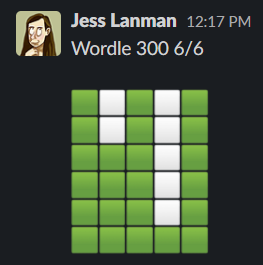
\includegraphics[width=0.2\linewidth]{pix/jess}\hfill\\
%%%DAVE CARD

		\vfill
		\begin{itemize}
			\item  Scrape Slack and Twitter for cards.
			\item Card are collected in a deck.
			\item The deck is then drawn from for a game.
		\end{itemize}
\end{frame}

%cards from scrape
	\begin{frame}
		\frametitle{Cardle}
		\hfill
		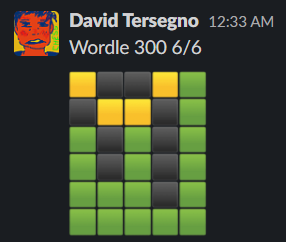
\includegraphics[width=0.2\linewidth]{pix/david}\hfill
		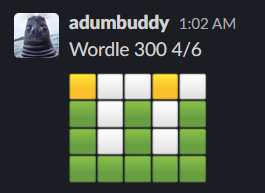
\includegraphics[width=0.2\linewidth]{pix/adam}\hfill
		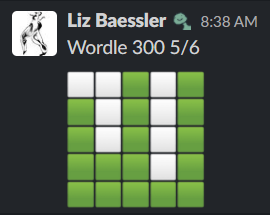
\includegraphics[width=0.2\linewidth]{pix/liz}\hfill
		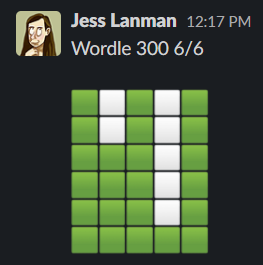
\includegraphics[width=0.2\linewidth]{pix/jess}\hfill\\
		%%%DAVE CARD
		
		\begin{center}
		\begin{tabular}{cccc}
	
		\begin{tabular}{|c|c|c|c|c|}
			\hline
			\cellcolor{yellow} & \cellcolor{gray}&\cellcolor{gray}&\cellcolor{yellow}&\cellcolor{green}\\
			\hline
			\cellcolor{gray}&\cellcolor{yellow}&\cellcolor{yellow}&\cellcolor{gray}&\cellcolor{green}\\
			\hline
			\cellcolor{green}&\cellcolor{gray}&\cellcolor{green}&\cellcolor{gray}&\cellcolor{green}\\
			\hline
			\cellcolor{green}&\cellcolor{gray}&\cellcolor{green}&\cellcolor{gray}&\cellcolor{green}\\
			\hline
			\cellcolor{green}&\cellcolor{green}&\cellcolor{green}&\cellcolor{gray}&\cellcolor{green}\\
			\hline
			\cellcolor{green}&\cellcolor{green}&\cellcolor{green}&\cellcolor{green}&\cellcolor{green}\\
			\hline
		\end{tabular}
	&
	%%%%% ADAM CARD
			\begin{tabular}{|c|c|c|c|c|}
			\hline
			\cellcolor{yellow} & \cellcolor{gray}&\cellcolor{gray}&\cellcolor{yellow}&\cellcolor{gray}\\
			\hline
			\cellcolor{green}&\cellcolor{gray}&\cellcolor{green}&\cellcolor{gray}&\cellcolor{green}\\
			\hline
			\cellcolor{green}&\cellcolor{gray}&\cellcolor{green}&\cellcolor{gray}&\cellcolor{green}\\
			\hline
			\cellcolor{green}&\cellcolor{green}&\cellcolor{green}&\cellcolor{green}&\cellcolor{green}\\
			\hline
		\end{tabular}
	&
				\begin{tabular}{|c|c|c|c|c|}
		\hline
		\cellcolor{gray} & \cellcolor{gray}&\cellcolor{green}&\cellcolor{gray}&\cellcolor{green}\\
		\hline
		\cellcolor{green}&\cellcolor{gray}&\cellcolor{green}&\cellcolor{gray}&\cellcolor{green}\\
		\hline
		\cellcolor{green}&\cellcolor{gray}&\cellcolor{green}&\cellcolor{gray}&\cellcolor{green}\\
		\hline
		\cellcolor{green}&\cellcolor{green}&\cellcolor{green}&\cellcolor{gray}&\cellcolor{green}\\
		\hline
		\cellcolor{green}&\cellcolor{green}&\cellcolor{green}&\cellcolor{green}&\cellcolor{green}\\
		\end{tabular}
&
\begin{tabular}{|c|c|c|c|c|}
	\hline
	\cellcolor{green} & \cellcolor{gray}&\cellcolor{green}&\cellcolor{gray}&\cellcolor{green}\\
	\hline
	\cellcolor{green}&\cellcolor{gray}&\cellcolor{green}&\cellcolor{gray}&\cellcolor{green}\\
	\hline
	\cellcolor{green}&\cellcolor{green}&\cellcolor{green}&\cellcolor{gray}&\cellcolor{green}\\
	\hline
	\cellcolor{green}&\cellcolor{green}&\cellcolor{green}&\cellcolor{gray}&\cellcolor{green}\\
	\hline
	\cellcolor{green}&\cellcolor{green}&\cellcolor{green}&\cellcolor{green}&\cellcolor{green}\\
\end{tabular}
\end{tabular}

\end{center}
%		\vfill
%		\begin{itemize}
%			\item <2-> Scrape Slack and Twitter for cards.
%			\item <3-> Generate a player's deck.
%		\end{itemize}
	\end{frame}

\begin{frame}
	\frametitle{Cardle}
	\begin{center}
		\begin{tabular}{ccccc}
			\begin{tabular}{|c|c|c|c|c|}
				\hline
				\cellcolor{yellow} & \cellcolor{gray}&\cellcolor{gray}&\cellcolor{yellow}&\cellcolor{green}\\
				\hline
				\cellcolor{gray}&\cellcolor{yellow}&\cellcolor{yellow}&\cellcolor{gray}&\cellcolor{green}\\
				\hline
				\cellcolor{green}&\cellcolor{gray}&\cellcolor{green}&\cellcolor{gray}&\cellcolor{green}\\
				\hline
				\cellcolor{green}&\cellcolor{gray}&\cellcolor{green}&\cellcolor{gray}&\cellcolor{green}\\
				\hline
				\cellcolor{green}&\cellcolor{green}&\cellcolor{green}&\cellcolor{gray}&\cellcolor{green}\\
				\hline
				\cellcolor{green}&\cellcolor{green}&\cellcolor{green}&\cellcolor{green}&\cellcolor{green}\\
				\hline
			\end{tabular}
		&
		+
		&
		\begin{tabular}{|c|c|c|c|c|}
			\hline
			\cellcolor{pink} & \cellcolor{gray}&\cellcolor{gray}&\cellcolor{pink}&\cellcolor{gray}\\
			\hline
			\cellcolor{purple}&\cellcolor{gray}&\cellcolor{purple}&\cellcolor{gray}&\cellcolor{purple}\\
			\hline
			\cellcolor{purple}&\cellcolor{gray}&\cellcolor{purple}&\cellcolor{gray}&\cellcolor{purple}\\
			\hline
			\cellcolor{purple}&\cellcolor{purple}&\cellcolor{purple}&\cellcolor{purple}&\cellcolor{purple}\\
			\hline
		\end{tabular}
	&
	=
	&
	\begin{tabular}{|c|c|c|c|c|}
		\hline
		\cellcolor{yellow} & \cellcolor{gray}&\cellcolor{gray}&\cellcolor{yellow}&\cellcolor{green}\\
		\hline
		\cellcolor{pink}&\cellcolor{yellow}&\cellcolor{yellow}&\cellcolor{pink}&\cellcolor{green}\\
		\hline
		\cellcolor{gray}&\cellcolor{gray}&\cellcolor{gray}&\cellcolor{gray}&\cellcolor{gray}\\
		\hline
		\cellcolor{gray}&\cellcolor{gray}&\cellcolor{gray}&\cellcolor{gray}&\cellcolor{gray}\\
		\hline
		\cellcolor{gray}&\cellcolor{gray}&\cellcolor{gray}&\cellcolor{purple}&\cellcolor{gray}\\
		\hline
		\cellcolor{green}&\cellcolor{green}&\cellcolor{green}&\cellcolor{green}&\cellcolor{green}\\
		\hline
	\end{tabular}
		\end{tabular}
	\end{center}
	
	\begin{itemize}
		\item Cards are overlaid to claim spaces on a 5$\times$6 grid.
		\item smaller cards have mores choices for where to place
		\item The board is populated with a player's colors, which add towards a final point value.
	\end{itemize}
\end{frame}

\begin{frame}\frametitle{Cardle}
	\begin{block}{pros}
		\begin{itemize}
			\small
			\item create different NNs to act as players. Perhaps one that can beat a human.
			\item classify players by type (unsupervised)
			\item quantitatively compare decks and strategies
			\item Make as much of my own data as I need by running and saving games on PC
			\item cards are already divided into players
			\item Slack and Twitter have reliable APIs to search for wordle grids
			\item cards and games statistics are easy to encode as arrays of integers.
			\item save many models as different players
			\item sounds like a lot of fun. I'm doing this eventually
		\end{itemize}
	\end{block}
	\begin{alertblock}{cons}
		\begin{itemize}
		\item 			\scriptsize{multiple NNs need to be run and trained on a very large data set before they start making good decisions}
		\item Implementing the game itself and a way for the models to interact with it will take some work.
		\item Entirely abstract. Doesn't show off NLP, regression unit interpretation
		\item regression methods limited
		\end{itemize}
	\end{alertblock}
\end{frame}


\begin{frame}
\frametitle{Longshot: Inscryption analytics}
\begin{center}
	\hfill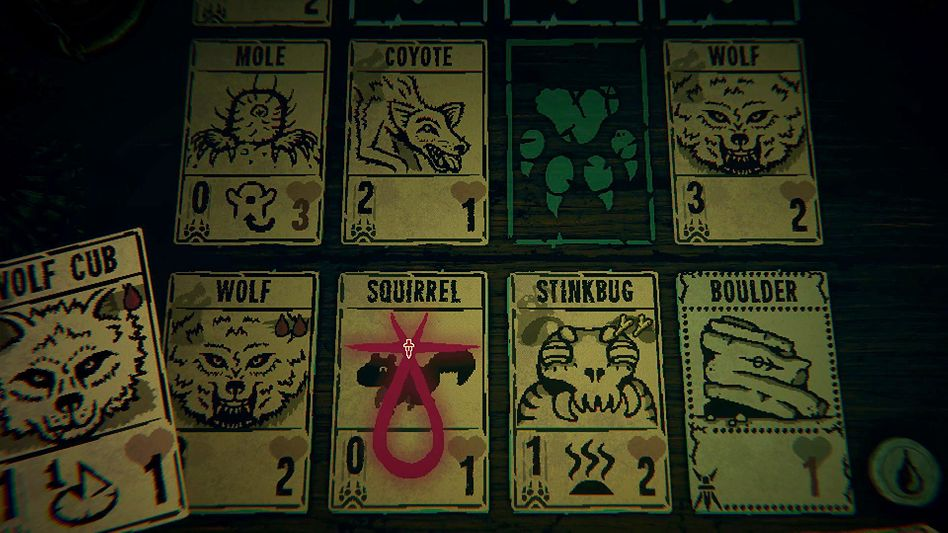
\includegraphics[width=0.5\linewidth]{pix/inscryption}\hfill
\includegraphics[width=0.3\linewidth]{pix/logo}\hfill
\end{center}
\begin{itemize}
	\item Analyze a deckbuilding video/card game with beta data on thousands of players
	\item Game is entirely discrete --- cards are placed in one of four positions, have easily enumerable, integer qualities.
	\item Quantitatively compare decks and strategies by success
	\item Build a model that can make informed decisions.
\end{itemize}
\end{frame}

\begin{frame}
	\frametitle{Longshot: Inscryption analytics}
	\begin{block}{pros}
		\begin{itemize}
			\item Use NNs, decision trees, or other to make player decisions
			\item identify pre-determined card types (wolf, insect, hooved, bird) as supervised learning
			\item identify player types as unsupervised
			\item Game is already divided into discrete steps and cards
			\item Data is already "useful" as it influenced the development
			\item sounds like a lot of fun
			\item active community
		\end{itemize}
	\end{block}
\begin{alertblock}{cons}
	\begin{itemize}
		\scriptsize
		\item Waiting to hear back from the developer and publisher. Good chance I wont hear from them.
		\item regression methods limited
		\item I could be in over my head with game analysis
	\end{itemize}
	\end{alertblock}
\end{frame}

	\begin{frame}
		\frametitle{Climate science literature review and meta-analysis}
		
		
		\begin{tabular}{cp{180pt}}
			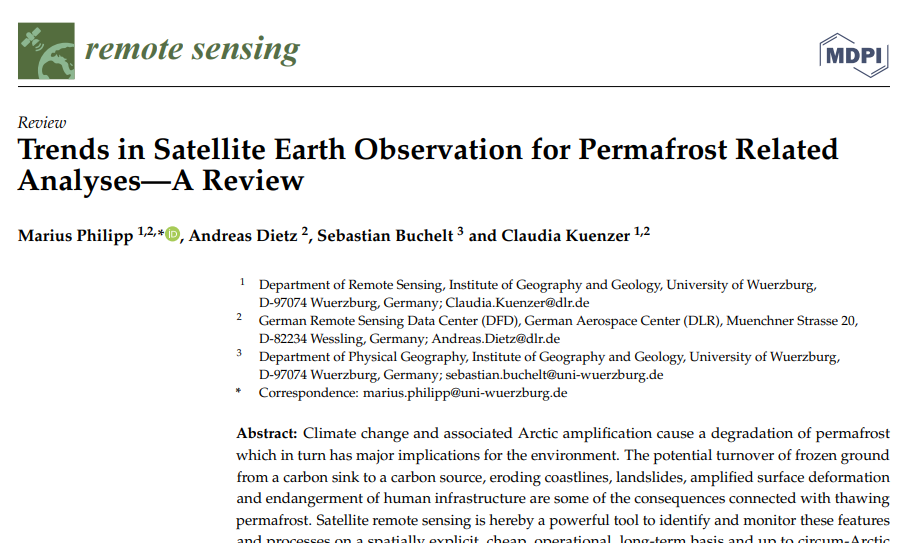
\includegraphics[width=0.5\linewidth, trim = 0 260pt 0 260pt]{pix/TrendsinSatelliteTitle}& $\bullet$ Literature review scraped for $>$500 \\ &\strut \qquad permafrost papers on remote\\
			& \strut \qquad sensing data since 2000\\
		& $\bullet$ Statistics on nationality and scientific impact (citations)\\
		& $\bullet$ correlations with local permafrost level
		\end{tabular}
	\end{frame}

	\begin{frame}
		\frametitle{Climate science literature review and meta-analysis}
		The goal: generate  numbers (regression coefficients) that reflect how effectively different groups of people will perform research and on which topics.
		\vfill \vfill\vfill
		\begin{tabular}{cp{0.5\linewidth}}
		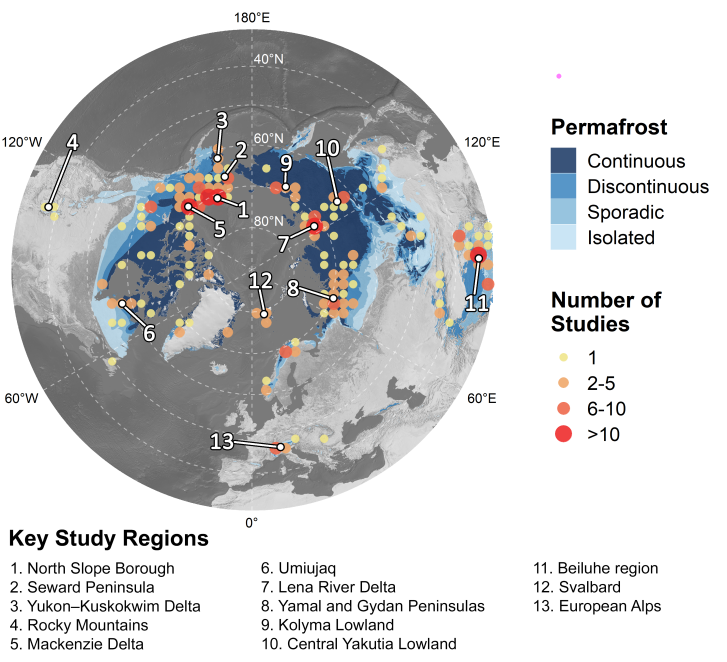
\includegraphics[width=0.5\linewidth, trim = 0 280pt 0 280pt]{pix/permamap}
		&-- Study could be duplicated for another topic:\\
		&$\bullet$ deforestation\\
		&$\bullet$ coral reef bleaching\\
		&$\bullet$ extreme weather\\
		&$\bullet$ desert expansion\\
		&$\bullet$ industrial pollution\\
	\end{tabular}

	\end{frame}

\begin{frame}\frametitle{Climate science literature review and meta-analysis}
	\begin{block}{pros}
		\begin{itemize}
			\item Shows off web scraping
			\item Uses regression
			\item could apply unsupervised classification to match "science types"
			\item The project is its own literature review.
			\item previous work in remote sensing
		\end{itemize}
	\end{block}
	\begin{alertblock}{cons}
		\begin{itemize}
			\item probably not "big data" ---  a statistically small number of scientifically active countries generating statistically small numbers of papers
			\item predictive and classification power may be limited
			\item will probably run into paywall problems.
		\end{itemize}
	\end{alertblock}
\end{frame}

\end{document}
